\section{The Non-interacting Case}

In the case of non-interacting particles, that is, the case with no electron-electron interaction, the trial wave function represents the exact wave function both in the case of quantum dots and atoms. For molecules and the double-well quantum dot, the additional requirement that $R\to\infty$ should also be applied, where $R$ is the distance between the atoms in the case of molecules, and the distance between the well centers in the case of the quantum dot. All of the presented systems are covered in detail in Chapter \ref{ch:modelledSystems}.

Exact solutions serve as a powerful guide, since results can be benchmarked against these, that is, the code can be validated. In the non-interacting case, Adaptive Stochastic Gradient Descent (ASGD) should always provide a variational parameter equal to unity, i.e.~$\alpha=1$. Variational Monte-Carlo (VMC) and Diffusion Monte-Carlo (DMC) should reproduce the exact solutions from Eq.~(\ref{eq:qdotsE0}) in the case of quantum dots and Eq.~(\ref{eq:atomsE0}) in the case of atomic systems to machine precision. 

In Table \ref{tab:res_valid_qdots}, validation runs for the three lowest lying closed-shell quantum dots are run for both two and three dimensions. Figure \ref{fig:ASGD_nonint} shows ASGD finding the exact minimum. Table \ref{tab:res_valid_atoms} shows similar results for atoms. As required, the closed form energies are reproduced to machine precision.

The double-well quantum dots results reproduce the non-interactive energies when the wells are placed far enough apart. This is demonstrated in Table \ref{tab:res_valid_qdots_doublewell}. A separation equal to $R = 20$ was sufficient. For molecules, on the other hand, the atomic nuclei interaction is very strong, implying the need of a greater separation of the atoms than what was needed for the wells. Table \ref{tab:res_valid_molecules} shows this effect; the convergence is nice for $\mathrm{H_2}$, however, for the heavier molecules, where the atomic nuclei interaction is higher, the convergence to the non-interacting limit is slower.

DMC should in the case of an exact wave function be perfectly stable. The trial energy should equal the ground state energy through all time steps and zero fluctuations in the number of walkers should occur. This trend is shown for the neon atom in Figure \ref{fig:DMC_neon_nonint}.

A final non-interacting case is run for DMC without the exact wave function. As discussed in Chapter \ref{ch:QMC}, DMC should result in a better estimate of the ground state energy than VMC in the case of a trial wave function which is different from the exact ground state. A test case is presented in Figure \ref{fig:DMC_nonExactWF}.

\setlength{\tabcolsep}{0.3cm}
\begin{table}[h]
\begin{center}
\begin{tabular}{c|cccccc||cccccc}
 & & & 2D & & & & & & & 3D \\
\hline
  $\omega$   & N & $\mathrm{E_{VMC}}$ & $\mathrm{E_{DMC}}$ & $\alpha$ & $E_0$ & \qquad  & \qquad &  N   & $\mathrm{E_{VMC}}$ & $\mathrm{E_{DMC}}$ & $\alpha$ & $E_0$ \\
\hline
 0.5 &   2   &   1.0    &   1.0    &   1.0    & 1  & \qquad & \qquad & 2     &   3.0   &   3.0    &   1.0    & 3 \\
 1.0 &       &   2.0    &   2.0    &   1.0    & 2  & \qquad & \qquad &       &   1.5   &   1.5    &   1.0    & 1.5 \\
 0.5 &   6   &   5.0    &   5.0    &   1.0    & 5  & \qquad & \qquad &  8    &   18.0  &   18.0   &   1.0    & 18 \\
 1.0 &       &   10.0   &   10.0   &   1.0    & 10 & \qquad & \qquad &       &  9.0    &   9.0    &   1.0    & 9 \\
 0.5 &   12  &   14.0   &   14.0   &   1.0    & 14 & \qquad & \qquad & 20    &  60.0   &   60.0   &   1.0    & 60 \\
 1.0 &       &   28.0   &   28.0   &   1.0    & 28 & \qquad & \qquad &       &  30.0   &   30.0   &   1.0    & 30 \\
\end{tabular}
\caption{Validation results for $N$-particle quantum dots with no Coulomb interaction and frequency $\omega$. The left-hand side shows the results for two dimensions, while the results for three dimensions are listed on the right-hand side. The last column for each dimension lists the exact energies $E_0$ calculated from Eq.~(\ref{eq:qdotsE0}). The exact solution to $\alpha$ is unity. As required, all methods reproduce the exact results. The variance is zero to machine precision for all listed results.}
\label{tab:res_valid_qdots}
\end{center}
\end{table}
\setlength{\tabcolsep}{6pt}

\setlength{\tabcolsep}{0.8cm}
\begin{table}[h]
\begin{center}
\begin{tabular}{cc|cccc}
  $\omega$   & N & $\mathrm{E_{VMC}}$ & $\mathrm{E_{DMC}}$ & $\alpha$ & $E_0(R\to\infty)$ \\
\hline
  0.5  &       &   4.0   & 4.0   &   1.0    & 4   \\
  1    &   4   &   2.0   & 2.0   &   1.0    & 2   \\
  0.5  &       &   20.0  & 20.0  &   1.0    & 20  \\
  1    &   12  &   10.0  & 10.0  &   1.0    & 10  \\
  0.5  &       &   28.0  & 28.0  &   1.0    & 28   \\
  1    &   24  &   56.0  & 56.0  &   1.0    & 56   \\
\end{tabular}
\caption{Validation results for $N$-particle double-well quantum dots with no Coulomb interaction and frequency $\omega$. The exact energy $E_0$, calculated from  Eq.~(\ref{eq:qdotsE0}), is listed in the last column. The calculations are performed with the wells separated at a distance $R=20$ in the $x$-direction. The exact solution to $\alpha$ is unity. As for the single-well quantum dots in Table \ref{tab:res_valid_qdots}, all methods reproduce the exact solution. The variance is zero to machine precision for all listed results. }
\label{tab:res_valid_qdots_doublewell}
\end{center}
\end{table}
\setlength{\tabcolsep}{6pt}

\setlength{\tabcolsep}{0.8cm}
\begin{table}
\begin{center}
\begin{tabular}{cc|cccc}
 Atom &   N     & $\mathrm{E_{VMC}}$ & $\mathrm{E_{DMC}}$ & $\alpha$ & $E_0$\\
\hline
 $\mathrm{He}$ &   2     &   -4.0   &   -4.0   &   1.0  & -4  \\
 $\mathrm{Be}$ &   4     &  -20.0   &  -20.0   &   1.0  & -20 \\
 $\mathrm{Ne}$ &   10    &  -200.0  &  -200.0  &   1.0  & -200\\
\end{tabular}
\caption{Validation results for different atoms consisting of $N$ electrons with no electron-electron Coulomb interaction. The exact energies $E_0$ are calculated from Eq.~(\ref{eq:atomsE0}). The exact solution of the variational parameter $\alpha$ is unity. As required, all methods reproduce the exact solutions. The variance is zero to machine precision for all listed results.}
\label{tab:res_valid_atoms}
\end{center}
\end{table}
\setlength{\tabcolsep}{6pt}

\setlength{\tabcolsep}{0.6cm}
\begin{table}
\begin{center}
\begin{tabular}{cc|cccc}
 Molecule &   N     & $R$ & $\mathrm{E_{VMC}}$ & $\mathrm{E_{DMC}}$ & $E_0(R\to\infty)$\\
\hline
 $\mathrm{H}_2$  & 2     & 10  &   -0.847    &  -0.9968    & -1  \\
   &       & 100  &  -0.979    &  -0.995  &  \\
   &       & 325   &  -1.000    &  -1.000  &  \\
 $\mathrm{Be}_2$  & 8     & 10  &  -41.596     &  -41.608   & -40 \\
  &        & 100 &  -40.298     &  -40.231   &     \\
   &       & 325 &  -40.123     &  -40.112   &     \\
 $\mathrm{Ne}_2$ &  20    & 10  &  -409.999    &  -410.010  & -400\\
  &        & 100 &  -401.390    &  -401.049  &     \\
  &        & 325 &  -           &  -         &     \\
\end{tabular}
\caption{Validation results for homonuclear diatomic molecules separated at a distance $R$ with no electron-electron interaction. The last column lists the exact energies $E_0$ calculated from Eq.~(\ref{eq:atomsE0}) for $R\to\infty$. Choosing $R$ too high results in a singular Slater determinant due to finite machine precision. This happens already for $R=325$ in the case of  $\mathrm{Ne}_2$. It is apparent that increasing $R$ brings the solutions closer to the exact energy. The statistical error is skipped.}
\label{tab:res_valid_molecules}
\end{center}
\end{table}
\setlength{\tabcolsep}{6pt}


\begin{figure}[h]
 \begin{center}
  \subfigure{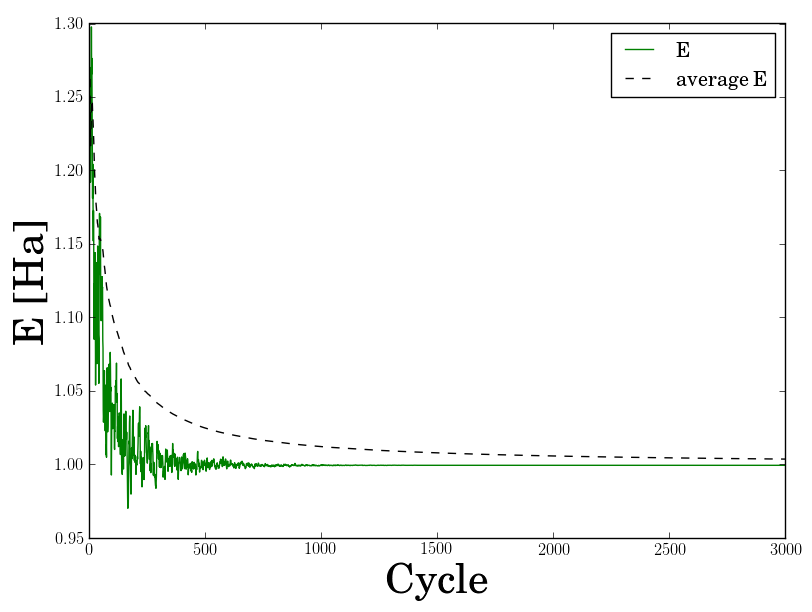
\includegraphics[scale=0.37]{../Graphics/ASGD_nonint_E.png}}
  \subfigure{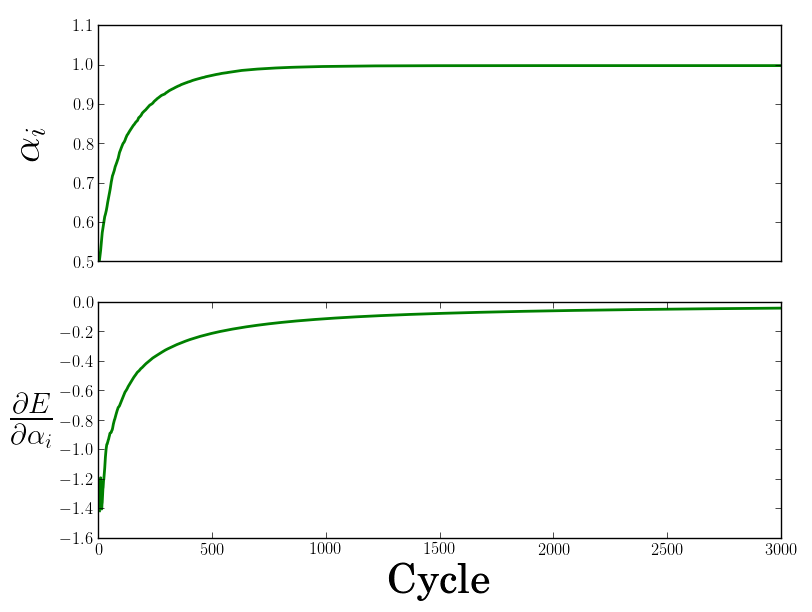
\includegraphics[scale=0.37]{../Graphics/ASGD_nonint.png}} 
  \caption{Adaptive Stochastic Gradient Descent (ASGD) results for a two-particle two-dimensional quantum dot with frequency $\omega=0.5$ and no electron-electron interaction. The exact energy $E_0=1$ is reached after approximately 1000 cycles, where the variational parameter $\alpha$ has converged close to unity. Due to enormous fluctuations the variational derivative is plotted as an accumulated average. The gradient is approximately zero after ~1000 cycles, in agreement with the behavior of the energy. The variational principle described in Section \ref{sec:selectingOptVarPar} is governing the trend of the energy convergence, however, a lot of statistical noise is present in the first 1000 cycles due to a high variance and a small number of samples.}
  \label{fig:ASGD_nonint}
 \end{center}
\end{figure}



\begin{figure}[h]
 \begin{center}
  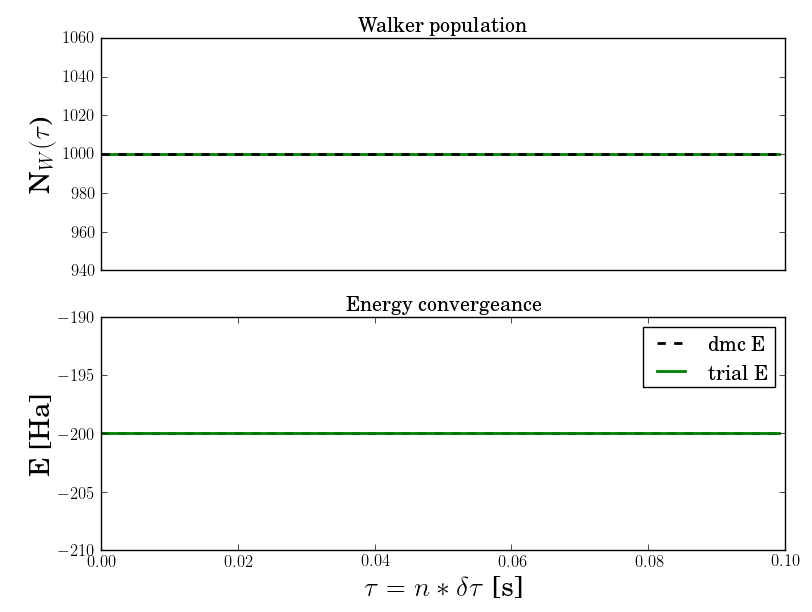
\includegraphics[scale=0.5]{../Graphics/DMC_neon_valid.png}
  \caption{Illustration of the Diffusion Monte-Carlo (DMC) energy convergence for the neon atom listed in Table \ref{tab:res_valid_atoms}. The trial energy is fixed at the exact ground state energy as required. The number of walkers are constant, implying an approximately zero variance in the samples.}
  \label{fig:DMC_neon_nonint}
 \end{center}
\end{figure}

\begin{figure}[h]
 \begin{center}
  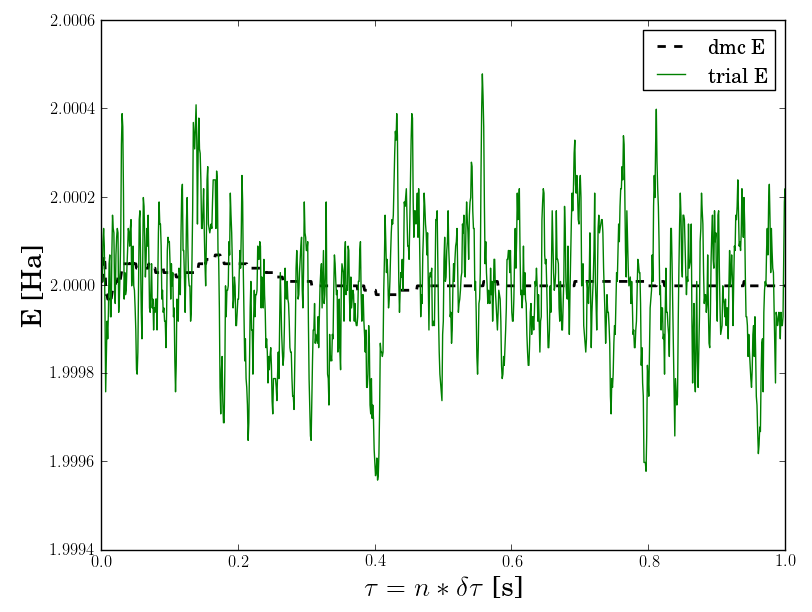
\includegraphics[scale=0.5]{../Graphics/DMC_notExactWF.png}
  \caption{Illustration of the Diffusion Monte-Carlo (DMC) energy convergence for a two-particle two-dimensional quantum dot with frequency $\omega=1$. The calculations are done with a variational parameter $\alpha=0.75$, where as the exact wave function is given for $\alpha=1$. Unlike the case with the exact wave function presented in Figure \ref{fig:DMC_neon_nonint}, the trial energy oscillates around the exact value $E_0 = 2.0$. The final result reveals a DMC energy of $2.00000(2)$, where the original Variational Monte-Carlo (VMC) energy was $2.0042(3)$. This illustrates the power of DMC contra VMC in the interesting cases where the exact wave function is unknown. The calculation was done using $10000$ random walkers.}
  \label{fig:DMC_nonExactWF}
 \end{center}
\end{figure}